
\chapter{Derivadas}

\PartialToc

\hypersetup{linkcolor=ptctitle}

\vspace*{0.5cm}
 
\begin{flushright}
\textit{\small{}El arte de nombrar y de medir con exactitud aquello
}\\
\textit{\small{} de lo que ni siquiera puede concebirse su existencia.}{\small{}
}\\
{\small{} Voltaire} 
\par\end{flushright}

\vspace*{-1mm}
 

\subsection{Introducción}

Los orígenes del Cálculo estuvieron motivados por el deseo de resolver
diversos problemas vinculados al movimiento de los cuerpos, así como
problemas de tipo geométrico de importancia en Óptica y problemas
de cálculo de valores máximos y mínimos de una función dada. Simplificando,
podemos destacar dos problemas principales: 
\begin{itemize}
\item[$\bullet$] Determinar la tangente a una curva en un punto (el problema de las
tangentes). 
\item[$\bullet$] Determinar el área encerrada por una curva (el problema de las cuadraturas). 
\end{itemize}
Son los conceptos de derivada e integral, respectivamente, los que
permiten resolver satisfactoriamente dichos problemas. Mientras que
el concepto de integral tiene sus raíces en la antigüedad clásica,
la otra idea fundamental del Cálculo, la derivada, no se formuló hasta
el siglo XVII. Fue el descubrimiento efectuado por Sir Isaac Newton
(1642 - 1727) y Gottfried Wilhelm Leibniz (1646 - 1716) de la relación
entre estas dos ideas, tan dispares en apariencia, lo que inició el
magnífico desarrollo del Cálculo. Si bien los trabajos de Newton y
Leibniz son decisivos por sus aportaciones e influencia, no hay que
olvidar que ellos son el punto culminante de un largo proceso en el
que han participado científicos de la talla de Johannes Kepler (1571
- 1630), René Descartes (1596 - 1650), Pierre de Fermat (1601 - 1665),
John Wallis (1616 -1703) e Isaac Barrow (1630 - 1677) entre otros.

\subsection{Concepto de derivada. Interpretación física y geométrica}

Para entender los resultados del Cálculo diferencial es necesario,
antes que nada, comprender la idea básica del mismo: el concepto de
derivada. La derivada de una función puede interpretarse geométricamente
como la pendiente de una curva, y físicamente como una razón ``instantánea''
de cambio. 

\subsection{Tangente a una curva}

En la primera mitad del siglo XVII no se conocían métodos generales
para calcular la tangente a una curva en un punto de la misma. Este
problema se presentaba con frecuencia en mecánica, en óptica y en
geometría, y generalmente se resolvía, de forma geométrica, con técnicas
adaptadas a cada caso particular. La dificultad está en que, siendo
la tangente una recta, se precisa conocer dos puntos de la misma,
o bien un punto y su pendiente, para poderla determinar.
\begin{figure}[H]
\centering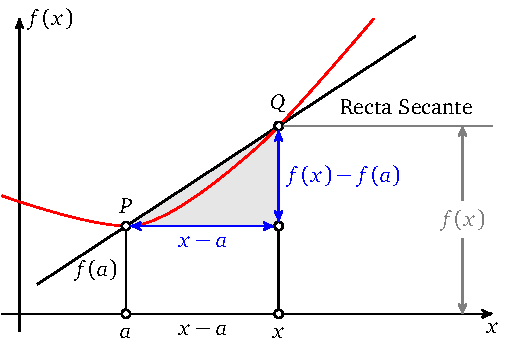
\includegraphics[scale=0.6]{20_home_antalcides_Calculo_pdf_derivada-1.pdf}\caption{Recta secante}
\label{sect}

\end{figure}

Supongamos que queremos hallar la tangente a una curva de ecuación
cartesiana $y=f(x)$ en el punto $(a,f(a))$. La estrategia, usada
primero por Pierre de Fermat y más tarde por Newton, consiste en aproximar
la tangente por rectas secantes cuyas pendientes sí pueden calcularse
directamente. En particular, consideremos la recta que une el punto
$(a,f(a))$ con un punto cercano, $(x,f(x))$, de la gráfica de $f$.
Esta recta se llama una secante (recta que corta a la curva, pero
no es tangente a la curva). La pendiente de esta secante es: 
\[
\frac{f(x)-f(a)}{x-a}
\]
dicho número suele llamarse \emph{cociente incremental de $f$ en
$a$}.

%\begin{floatingfigure}{95cm}%\flushleft 

%\caption{Recta secante}
%\label{sect}
%\end{floatingfigure}

Observa que una secante es una buena aproximación de la tangente,
siempre que el punto $Q(x,f(x))$ esté próximo al punto $P(a,f(a))$.
Estas consideraciones llevan a \emph{definir la tangente a la gráfica
de $f$ en el punto $P(a,f(a))$ como la recta que pasa por dicho
punto y cuya pendiente es igual al límite}: 
\[
\lim_{x\to a}\frac{f(x)-f(a)}{x-a}
\]
supuesto, claro está, que dicho límite exista. 

\subsection{Razón de cambio puntual y velocidad instantánea}

Muchas leyes de la Física, la Química, la Biología o la Economía,
son funciones que relacionan una variable ``dependiente'' $y$ con
otra variable ``independiente'' $x$, lo que suele escribirse en
la forma $y=f(x)$. Si la variable independiente cambia de un valor
inicial $a$ a otro $x$, la variable $y$ lo hace de $f(a)$ a $f(x)$.
La \emph{razón de cambio promedio de $y=f(x)$ con respecto a $x$
en el intervalo $[a,x]$} es: 
\[
\textrm{Razón de cambio promedio\ }=\frac{f(x)-f(a)}{x-a}
\]
Con frecuencia interesa considerar la razón de cambio en intervalos
cada vez más pequeños. Esto lleva a definir lo que podemos llamar
``\emph{razón de cambio puntual de $y=f(x)$ con respecto a $x$
en el punto $a$}'' como: 
\[
\lim_{x\to a}\frac{f(x)-f(a)}{x-a}.
\]
El ejemplo más conocido de esto que decimos es el de un móvil que
se mueve a lo largo de una recta sobre la cual hemos elegido un origen.
Sea $s(t)$ la posición del móvil en el tiempo $t$, es decir, la
distancia con signo del móvil al origen en el tiempo $t$. La razón
de cambio promedio tiene en este caso una interpretación física natural:
\[
\frac{s(a+h)-s(a)}{h}
\]
Es la \emph{velocidad media} del móvil en el intervalo de tiempo comprendido
entre $a$ y $a+h$. Parece intuitivo que, en cada instante, el móvil
se mueve con una determinada \emph{velocidad instantánea}. Pero no
hay manera de medir directamente una velocidad instantánea; un instante
quiere decir una posición en la recta: la velocidad instantánea del
móvil para $t=a$ es la velocidad que tiene cuando está en la posición
$s(a)$. La velocidad instantánea es una abstracción de un característica
física del movimiento, pero no es una magnitud que podamos observar
directamente. La única definición razonable de velocidad instantánea
es como la razón de cambio puntual: 
\[
\lim_{h\to0}\frac{s(a+h)-s(a)}{h}
\]

\noindent \textbf{Notación}.\ En lo que sigue usaremos las letras
$I$, $J$ para representar intervalos no vacíos de números reales.

\begin{defi}{Derivada en un punto}{def}\label{def:derivada} Se dice
que una función \func{f}{I}\ es \textbf{derivable en un punto
$a\in I$}, si existe el límite: 
\[
\lim_{x\to a}\frac{f(x)-f(a)}{x-a}.
\]
Explícitamente, $f$ es derivable en $a$ si hay un número $L\in\R$
verificando que para cada número $\varepsilon>0$ existe algún número
$\delta>0$ tal que para todo $x\in I$ con $x\neq a$ y %
\mbox{%
$\mid x-a\mid<\delta$%
} se tiene que: 
\[
\left|\frac{f(x)-f(a)}{x-a}\ -\ L\right|\leqslant\varepsilon.
\]
Dicho número $L$ se llama \textbf{derivada de $f$ en $a$} y lo
representaremos por $f\tl(a)$ (notación debida a Lagrange). \end{defi}

\begin{defi}{Derivada de una función}{} Dada una función $f:I\rightarrow\R$
derivable en todo punto de $I$, la \textbf{función derivada} de $f$
es la función $f\tl:I\rightarrow\R$ que a cada punto $x\in I$ hace
corresponder la derivada de $f$ en dicho punto. \end{defi}

\begin{ideabox}\label{ob:propiedadlocalderivada} \textbf{i)}\ El
límite $\ {\displaystyle \lim_{x\to a}\frac{f(x)-f(a)}{x-a}}$ se
puede escribir también de la forma $\ {\displaystyle \lim_{h\to0}\frac{f(a+h)-f(a)}{h}.}$

\noindent \textbf{ii)}\ La derivabilidad de $f$ en un punto $a\in I$
es una \emph{propiedad local}, depende solamente del comportamiento
de $f$ en los puntos de $I$ próximos al punto $a$. Concretamente,
si $J$ es cualquier \emph{intervalo abierto} que contiene el punto
$a$, se verifica que $f$ es derivable en $a$ si, y sólo si, la
función restricción $f_{|I\cap J}$ es derivable en $a$ y, por supuesto,
en tal caso ambas funciones tienen la misma derivada en $a$. \end{ideabox}

\noindent \textbf{La notación diferencial de Leibniz.}\ La notación
$\dfrac{\df{f(x)}}{\df{x}}$ para representar la derivada de $f$
en $x$ es debida a Leibniz.

Leibniz interpretaba ese símbolo como un ``cociente diferencial''
pues él lo entendía así: como un cociente de cantidades infinitesimales,
y lo manejaba como un cociente; por ejemplo, se puede multiplicar
o dividir, según convenga, por $\df{x}$ o $\df{f(x)}$. En el capítulo
5 hemos visto los problemas que planteaba el uso de cantidades infinitesimales,
y cómo, finalmente, a partir del último tercio del siglo XIX, fueron
totalmente abandonadas. Por eso, la interpretación de Leibniz de la
derivada, aunque intuitiva, no es la que se sigue en la gran mayoría
de los cursos de cálculo\footnote{Aunque sí en los cursos de Análisis No Estándar basados en los hiperreales
de A. Robinson.}.

A pesar de lo dicho, es frecuente, sobre todo en libros de ingeniería,
usar la notación de Leibniz y manejarla como él lo hacía. Creo que
esto es útil porque la notación de Leibniz tiene una gran fuerza heurística,
y no debe presentar ningún problema, siempre que no acabes creyendo
que una derivada, tal como la hemos definido, es un cociente de infinitésimos.
Y siempre que dicha notación se use como un mero simbolismo y no se
hagan demostraciones apoyadas en su supuesta significación.

Una dificultad de la notación de Leibniz es que no es cómoda para
representar la derivada en un punto concreto. Podemos entender que
$\dfrac{\df{f(x)}}{\df{x}}$ es la función derivada $f\tl(x)$, pero
¿cómo indicamos la derivada en punto concreto $a$? Las notaciones
$\dfrac{\df{f(a)}}{\df{x}}$ y $\dfrac{\df{f(x)}}{\df{x}}(a)$ son
confusas. Lo que suele hacerse es escribir: 
\[
\left.\dfrac{\df{f(x)}}{\df{x}}\right|_{x=a}
\]
que, realmente, es una notación incómoda. Una posible mejora sería
escribir $\dfrac{\df{f}}{\df{x}}(x)$ para representar $f\tl(x)$,
en cuyo caso $\dfrac{\df{f}}{\df{x}}(a)$ indicaría $f\tl(a)$.

La verdad es que la mayoría de los libros de ingeniería que usan estas
notaciones lo hacen sin preocuparse mucho por su significado, y esa
es una causa importante de que muchas veces no se entienda bien lo
que escriben. Las notaciones son importantes y hay que manejarlas
cuidadosamente. Y todavía más, cuando una notación se supone que tiene
un significado casi mágico, y que por su fuerza simbólica ella sola,
por sí misma, proporciona demostraciones. Volveremos a considerar
este asunto más adelante.

\begin{defi}{Recta tangente}{} Supuesto que $f$ es derivable en
$a$, la recta de ecuación cartesiana: 
\[
y=f(a)+f\tl(a)(x-a)
\]
se llama \textbf{recta tangente} a la gráfica de $f$ en el punto
$(a,f(a))$, y también recta tangente a $f$ en $x=a$.

Cuando $f\tl(a)\neq0$, la recta de ecuación: 
\[
y=f(a)-\dfrac{1}{f\tl(a)}(x-a)
\]
es la \textbf{recta normal} a la gráfica de $f$ en el punto $(a,f(a))$,
y también recta normal a $f$ en $x=a$ \end{defi}

\subsubsection{Elementos de una curva relacionados con la derivada}

En la figura~\ref{figcurva} se han representado algunos elementos
de una curva que se expresan por medio de la derivada.

\begin{figure}[H]
\centering 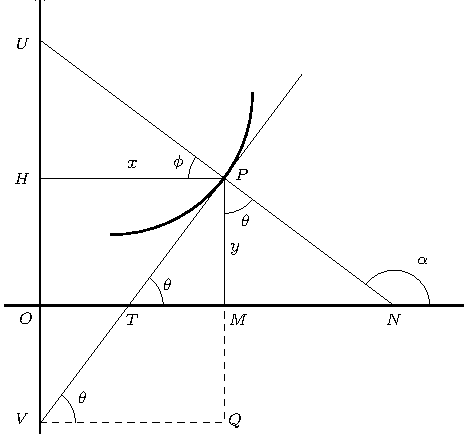
\includegraphics[scale=0.8]{21_home_antalcides_Calculo_pdf_rtan.pdf}\caption{\label{figcurva}{\small{}{Elementos de una curva relacionados con
la derivada}}}
\end{figure}

\begin{itemize}
\item La pendiente de la tangente es $\tg(\theta)=y\tl$. 
\item La pendiente de la normal es $\tg(\alpha)=\tg(\pi/2+\theta)=-1/y\tl$. 
\item El segmento $\overline{TM}$ es la \textbf{subtangente}. Su longitud
viene dada por $\overline{TM}=y\cotg(\theta)=y/y\tl$. 
\item El segmento $\overline{MN}$ es la \textbf{subnormal}. Su longitud
viene dada por $\overline{MN}=y\tg(\theta)=yy\tl$. 
\item Los segmentos interceptados en los ejes $OX$ y $OY$ por la tangente
son 
\[
\begin{cases}
\overline{OT}=\overline{OM}-\overline{TM}=x-y/y\tl\\
\overline{OV}=\overline{PM}-\overline{PQ}=y-x\tg(\theta)=y-xy\tl
\end{cases}
\]
\item Los segmentos interceptados en los ejes $OX$ y $OY$ por la normal
son 
\[
\begin{cases}
\overline{ON}=\overline{OM}+\overline{MN}=x+y\tg(\theta)=x+yy\tl\\
\overline{OU}=\overline{OH}+\overline{HU}=y+x\tg(\phi)=y+x\tg(\pi/2-\theta)=y+x/y\tl
\end{cases}
\]
\end{itemize}

\subsection{Derivadas laterales}

\begin{defi}{Derivadas laterales}{} Se dice que $f$ es \textbf{derivable
por la izquierda en $a$} si existe el límite: 
\[
\lim_{\substack{x\to a\\
x<a
}
}\frac{f(x)-f(a)}{x-a}.
\]
El valor de dicho límite se llama la \textbf{derivada por la izquierda}
de $f$ en $a$.

Análogamente se dice que $f$ es \textbf{derivable por la derecha
en $a,$} si existe el límite: 
\[
\lim_{\substack{x\to a\\
x>a
}
}\frac{f(x)-f(a)}{x-a}.
\]
El valor de dicho límite se llama la \textbf{derivada por la derecha}
de $f$ en $a$. \end{defi}

Teniendo en cuenta la relación que hay entre el límite de una función
en un punto y los límites laterales, es claro que: 
\begin{itemize}
\item[i)] Si $a=\max I$, entonces la derivabilidad de $f$ en $a$ es lo mismo
que la derivabilidad por la izquierda de $f$ en $a$. 
\item[ii)] Si $a=\min I$, entonces la derivabilidad de $f$ en $a$ es lo mismo
que la derivabilidad por la derecha de $f$ en $a$. 
\item[iii)] Si $a$ no es un extremo de $I$, entonces equivalen las afirmaciones: 
\begin{itemize}
\item[a)] $f$ es derivable en $a$. 
\item[b)] Las derivadas por la izquierda y por la derecha de $f$ en $a$ existen
y coinciden. 
\end{itemize}
\end{itemize}

\subsection{Propiedades de las funciones derivables. Reglas de derivación}

El siguiente resultado nos dice que la derivabilidad es una propiedad
más fuerte que la continuidad.

\begin{proposicion}{}{} Toda función derivable en un punto es continua
en dicho punto. \end{proposicion}

\begin{prueba} En efecto, si \func{f}{I}\ es derivable en $a$,
de la igualdad: 
\[
f(x)=f(a)+(x-a)\frac{f(x)-f(a)}{x-a}\quad(x\en I,\ x\neq a)
\]
se sigue que $\dis\lim_{x\to a}f(x)=f(a)$, es decir, $f$ es continua
en $a$.\end{prueba}

\begin{teo}{Reglas de derivación}{}\ Sean \func{f,g}{I}\ dos
funciones. Se verifican las siguientes afirmaciones: 
\begin{itemize}
\item[i)] La funciones suma, $f+g$, y producto, $fg$, son derivables en todo
punto $a\en I$ en el que $f$ y $g$ sean derivables, y las derivadas
respectivas vienen dadas por:

\[
(f+g)^{\prime}(a)=f\tl(a)+g\tl(a);\quad(fg)^{\prime}(a)=f\tl(a)g(a)+f(a)g\tl(a)
\]

\item[ii)] Si $g(x)\neq0$ para todo $x\in I$, la función cociente $f/g$ es
derivable en todo punto $a\en I$ en el que $f$ y $g$ sean derivables,
en cuyo caso se verifica que: 
\[
\left(\frac{f}{g}\right)^{\prime}(a)=\frac{f\tl(a)g(a)-f(a)g\tl(a)}{(g(a))^{2}}
\]
\end{itemize}
\end{teo} 

\begin{prueba} Las reglas de derivación se prueban muy fácilmente
haciendo uso de las propiedades algebraicas de los límites y la definición
de derivada. Es suficiente que tengas en cuenta las siguientes igualdades:
\begin{eqnarray*}
\dfrac{(f+g)(x)-(f+g)(a)}{x-a} & = & \dfrac{f(x)-f(a)}{x-a}+\dfrac{g(x)-g(a)}{x-a}\\
\dfrac{(fg)(x)-(fg)(a)}{x-a} & = & \dfrac{f(x)-f(a)}{x-a}g(x)+f(a)\dfrac{g(x)-g(a)}{x-a}\\
\dfrac{\frac{1}{g}(x)-\frac{1}{g}(a)}{x-a} & = & -\dfrac{g(x)-g(a)}{x-a}\dfrac{1}{g(x)g(a)}
\end{eqnarray*}
De la primera y segunda igualdades se deduce, tomando límites para
$x\to a$ , las reglas para la derivada de una suma y de un producto.
Igualmente, de la tercera igualdad, se deduce la derivada de $\frac{1}{g}$,
de donde, se obtiene la derivada de $\frac{f}{g}=f\frac{1}{g}$ haciendo
uso de la regla para derivar un producto.\end{prueba}

Como las funciones constantes tienen derivada nula en todo punto y
la función identidad, $f(x)=x$, tiene derivada igual a 1 en todo
punto, aplicando las reglas de derivación anteriores se obtiene el
siguiente corolario.

\begin{coro}{}{} Las funciones polinómicas son derivables en todo
punto y las funciones racionales son derivables en todo punto de su
conjunto natural de definición. Además la derivada de la función polinómica
\mbox{%
$\ f(x)=a_{0}+a_{1}x+a_{2}x^{2}+\cdots+a_{n}x^{n}$\ %
} en cada punto $x\in\R$ viene dada por: 
\[
f\tl(x)=a_{1}+2a_{2}x+3a_{3}x^{2}+\cdots+na_{n}x^{n-1}
\]
\end{coro}

\begin{teo}{Derivación de una función compuesta o regla de la cadena}{}{}

Sean \func{f}{I}\ y \func{g}{J}\ con $f(I)\subset J$,
y sea \func{h=g\!\circ \!f}{I}\ la función compuesta. Supongamos
que $f$ es derivable en $a\en I$ y que $g$ es derivable en $f(a)$.
Entonces $h$ es derivable en $a$ y $h\tl(a)=g\tl(f(a))f\tl(a)$.

\noindent En particular, si $g$ es derivable en $J$, la función
compuesta $h=g\!\circ\!f$ es derivable en todo punto de $I$ donde
$f$ sea derivable. \end{teo}

\noindent \begin{prueba} Pongamos $b=f(a)$. Tenemos que probar que
$\dis{\lim_{x\to a}\frac{h(x)-h(a)}{x-a}=g\tl(b)f\tl(a)}$. Por hipótesis
se cumple que :
\[
\lim_{y\to b}\frac{g(y)-g(b)}{y-b}\lim_{x\to a}\frac{f(x)-f(a)}{x-a}=g\tl(b)f\tl(a)
\]
La idea de la demostración es hacer en esta igualdad la sustitución
$y=f(x)$. Como no está garantizado por las hipótesis hechas que para
$x\neq a$ se tenga %
\mbox{%
$f(x)\neq b$,%
} no está justificado hacer directamente la sustitución indicada (dividir
por cero está prohibido). Podemos evitar esta dificultad como sigue.
Definamos la función \func{\ff}{J}\ por: 
\[
\ff(y)=\frac{g(y)-g(b)}{y-b}\ \ (y\neq b),\ \ff(b)=g\tl(b)
\]
Con ello la función \ff\ es continua en $b$. Es inmediato ahora
comprobar que para todo $x\en I$ con $x\neq a$ se verifica que:
\begin{equation}
\frac{h(x)-h(a)}{x-a}=\ff(f(x))\frac{f(x)-f(a)}{x-a}.\label{equality}
\end{equation}
Ahora, como $f$ es continua en $a$ (porque es derivable en $a$)
y \ff\ es continua en $b=f(a)$, se sigue que $\ff\circ f$ es continua
en $a$, por lo que: 
\[
\lim_{x\to a}\ff(f(x))=\ff(f(a))=\ff(b)=g\tl(b).
\]
La igualdad (\ref{equality}) nos dice ahora que:
\[
\lim_{x\to a}\frac{h(x)-h(a)}{x-a}=g\tl(b)f\tl(a)
\]
como queríamos probar.\end{prueba}

\noindent \textbf{Regla de la cadena al estilo Leibniz.} Una demostración
de la regla de la cadena al ``estilo Leibniz'' podría ser como sigue.
Por una parte, tenemos que $y$ es función de $x$ a través de $g$,
es decir, $y=g(x)$. También tenemos que $x$ es función de $t$ a
través de $f$, $x=f(t)$. Entonces la variación de $y$ respecto
a $t$ se hace por intermedio de $x$: 
\begin{equation}
\frac{\df{y}}{\df{t}}=\frac{\df{y}}{\df{x}}\frac{\df{x}}{\df{t}}\label{cadenaleibniz}
\end{equation}
Hemos acabado. Todo lo que hemos hecho ha sido multiplicar y dividir
por $\df{x}$.

No sé lo que pensará tú de esto, pero a mí me parecería una broma
que alguien pretendiera que lo que hemos hecho es una demostración.
Primero: ¿qué es $\df{x}$? Porque si es un símbolo, no tiene sentido
multiplicar y dividir por él (salvo que a esta operación se le hubiera
asignado previamente un significado preciso) y si es un número ¿cómo
está definido? ¿qué relación tiene ese número con la derivada? Preguntas
sin respuesta. A esto me refería al decir que una notación, por sí
sola, no sirve para demostrar nada.

Además, el simbolismo empleado en la igualdad (\ref{cadenaleibniz})
no indica dónde se evalúa cada una de las derivadas, y eso es fundamental
para entender la regla de la cadena. Fíjate que la regla de la cadena
nos dice que la derivada de una función compuesta de dos funciones
derivables, $h(x)=(g\circ f)(x)$, viene dada por 
\begin{equation}
h\tl(x)=g\tl(f(x))f\tl(x)=(g\tl\circ f)(x)f\tl(x)\label{cadenalagrange}
\end{equation}
que es un producto de dos funciones, $g\tl(f(x))$ y $f\tl(x)$, pero
la primera de ellas $g\tl(f(x))=(g\tl\circ f)(x)$ es una \emph{función
compuesta}. Por eso si queremos volver a derivar en la igualdad (\ref{cadenalagrange}),
debemos aplicar la regla para derivar un producto y, para derivar
el primer factor, debemos aplicar la regla de la cadena. Es por eso
que, en la regla de la cadena, es fundamental indicar los puntos donde
se evalúan las derivadas.

La notación en la igualdad (\ref{cadenaleibniz}) es mala porque no
indica dónde se evalúa cada una de las derivadas. Pero también es
mala por las razones siguientes.

$\bullet\quad$Una misma letra representa dos funciones distintas.
En (\ref{cadenaleibniz}) la letra $y$ aparece a la izquierda y a
la derecha. A la izquierda representa la función compuesta $y=g(f(t))$,
a la derecha representa la función $y=g(x)$.

\indent$\bullet\quad$Una misma letra representa una función y una
variable. La letra $x$ en la parte derecha representa la variable
en $y=g(x)$, y también representa la función $x=f(t)$.

Demasiado confuso ¿verdad? A pesar de lo dicho, la igualdad (\ref{cadenaleibniz})
aparece en muchos textos de matemáticas para ingenieros y en textos
de física, sin ningún comentario, sin explicar lo que significa y
pretendiendo que constituye por sí misma una demostración. Lo peor
de todo, es que si te la enseñan así puedes creer que la entiendes,
y entonces una de dos: o la entiendes de verdad, como acabo de explicarlo,
o te engañas y realmente no sabes lo que crees saber. Lamentablemente,
de estas dos posibilidades la más frecuente es la segunda.

Y…sin embargo, la igualdad (\ref{cadenaleibniz}) es muy simple y
fácil de recordar, y permite conjeturar la regla de la cadena sin
necesidad de demostrarla (por eso decimos que la notación de Leibniz
tiene un gran valor heurístico). Mi consejo es el siguiente: puedes
usar la notación de Leibniz siempre que te ayude en lo cálculos, pero
no debes dejarte llevar por la notación sino que debes entender lo
que estás haciendo en cada momento.

\begin{ejemplo} Sabiendo que $y=\sen x$ y $x=\cos t$, se pide calcular
la derivada de $y$ con respecto a $t$.

Lo que nos piden es calcular la derivada de la función compuesta $h(t)=\sen(\cos t)$.
Aquí $g(x)=\sen x$, $f(t)=\cos t$. Tenemos que 
\[
h\tl(t)=g\tl(f(t))f\tl(t)=-\cos(\cos t)\sen t
\]
Al estilo Leibniz: 
\[
\frac{\df{y}}{\df{t}}=\frac{\df{y}}{\df{x}}\frac{\df{x}}{\df{t}}=\cos x(-\sen t)=-\cos x\sen t
\]
Pero esta igualdad debe ser función de $t$ por lo que hay que sustituir
$x=\cos t$ y se vuelve a obtener el resultado anterior. \end{ejemplo}

\subsection{Derivación implícita}

\subsection{Derivada de la la función inversa}

\subsection{Derivabilidad de las funciones Transcendentales}

\subsubsection{Derivabilidad de la exponencial y del logaritmo. Criterio de equivalencia
logarítmica}

Aceptaremos que las funciones logaritmo, exponencial, trigonométricas
y sus inversas, son derivables, pues ahora no sería fácil probarlo.
Más adelante dispondremos de herramientas para hacerlo con comodidad.

La función exponencial $x\mapsto\exp(x)=\e^{x}$, $(x\in\R)$, y la
función logaritmo natural %
\mbox{%
$x\mapsto\log x$%
}, $(x\in\R^{+})$, son derivables en todo punto de sus respectivos
intervalos de definición, siendo: 
\[
(\exp)^{\prime}(x)=\exp x\ \ensuremath{\forall x\in\R),\ \ \ \ (\log)^{\prime}(x)=\frac{1}{x}\ \ensuremath{\forall x\in\R^{+})}}
\]
En particular, se verifica que: 
\[
\dis{\lim_{x\to1}\frac{\log x}{x-1}=1;\quad\lim_{x\to0}\frac{\e^{x}-1}{x}=1;\quad\lim_{x\to0}\frac{\log(1+x)}{x}=1;\quad\lim_{x\to0}(1+x)^{1/x}=\e}
\]
Pues los primeros tres límites son derivadas y el cuarto se reduce
fácilmente al tercero. Deducimos también un importante resultado que
permite resolver en muchos casos las indeterminaciones ``$1^{\infty}$''
y ``$0\infty$''.

\begin{teo}{Criterio de equivalencia logarítmica}{}\label{zapato}
Sea $a\en I$, $f$ y $g$ funciones definidas en %
\mbox{%
$I\setminus\{a\}$.%
} Supongamos que $f(x)>0$ para $x\en I\setminus\{a\}$, y que $\dis\lim_{x\to a}f(x)=1$.
Entonces se tiene que: 
\begin{itemize}
\item[i)] $\dis\lim_{x\to a}f(x)^{g(x)}=\e^{L}\ $ si, y sólo si, $\dis\lim_{x\to a}g(x)(f(x)-1)=L$. 
\item[ii)] $\dis\lim_{x\to a}f(x)^{g(x)}=+\infinity\ $ si, y sólo si, $\dis\lim_{x\to a}g(x)(f(x)-1)=+\infinity$. 
\item[iii)] $\dis\lim_{x\to a}f(x)^{g(x)}=0\ $ si, y sólo si, $\dis\lim_{x\to a}g(x)(f(x)-1)=-\infinity$. 
\end{itemize}
\end{teo} \dem Sea \func{\ff}{\Rp}\ la función dada por:
\[
\ff(x)=\frac{\log x}{x-1},\ (x\neq1),\ \ff(1)=1.
\]
Nótese que \ff\ es una función continua. Pongamos: 
\[
f(x)^{g(x)}=\exp\big(g(x)\log(f(x))\big)=\exp\big(g(x)(f(x)-1)\ff(f(x))\big)
\]
Puesto que $\dis\lim_{x\to a}\ff(f(x))=1$ se sigue que: 
\[
\lim_{x\to a}g(x)(f(x)-1)\ff(f(x))=L\en\R\cup\{+\infinity\}\cup\{-\infinity\}
\]
si, y sólo si 
\[
\lim_{x\to a}g(x)(f(x)-1))=L\en\R\cup\{+\infinity\}\cup\{-\infinity\}
\]
lo que prueba las afirmaciones hechas.\fin

Las afirmaciones que se hacen en la siguiente proposición son consecuencia
fácil de la regla de la cadena.

\begin{proposicion}{}{} Sean $f,g:I\rightarrow\R$, $a\en I$ y $g(x)>0$
para todo $x\in I$. Se verifica entonces que:\\
i) $f$ es derivable en $a$ si, y sólo si, la función $h(x)=\exp(f(x))$
es derivable en $a$ en cuyo caso $\ h^{\prime}(a)=f\tl(a)\exp(f(a))$.\\
ii) $g$ es derivable en $a$ si, y sólo si, la función $\varphi(x)=\log(g(x))$
es derivable en $a$ en cuyo caso ${\ {\displaystyle \varphi\tl(a)=\frac{g\tl(a)}{g(a)}.}}$\\
iii) Si $f$ y $g$ son derivables en $a$ la función $\psi(x)=g(x)^{f(x)}$
también es derivable en $a$ y 
\[
\psi\tl(a)=\psi(a)\left(\log(g(a))f\tl(a)+f(a)\frac{g\tl(a)}{g(a)}\right)
\]
\end{proposicion}

Te recuerdo que una forma cómoda para trabajar con funciones de la
forma $\psi(x)=g(x)^{f(x)}$ es escribirlas como exponenciales $\psi(x)=\exp\big(f(x)\log(g(x))\big)$.\vspace*{-3mm}


\subsubsection{Derivación logarítmica}

\subsubsection{Derivabilidad de las funciones trigonométricas}

Las funciones seno y coseno son derivables en todo punto verificándose
que: 
\[
\sen\tlo(x)=\cos x\quad\cos\tlo(x)=-\sen x.
\]
En particular, se verifica que: 
\[
\lim_{x\to0}\dfrac{\sen x}{x}=1,\quad\lim_{x\to0}\dfrac{\cos x-1}{x}=0.
\]
Las derivadas de las demás funciones trigonométricas se deducen con
facilidad a partir de las derivadas del seno y del coseno. \vspace*{-3mm}


\subsubsection{Derivabilidad de las funciones hiperbólicas}

Las derivadas de las funciones hiperbólicas y de sus inversas se deducen
con facilidad de las derivadas del logaritmo y de la exponencial.
Se comprueba sin dificultad que 
\[
\senh\tlo(x)=\cosh x,\quad\cosh\tlo(x)=\senh x
\]
Las derivadas de las funciones hiperbólicas inversas son muy útiles
para calcular primitivas de funciones en las que intervienen raíces
cuadradas de trinomios de segundo grado. 
\begin{center}
\begin{tabular}{|c|c|}
\hline 
% after \\: \hline or \cline{col1-col2} \cline{col3-col4} ...
\raisebox{1em}{$\rule{0mm}{9mm}\dis\argsenh(x)=\log\left(x+\sqrt{x^{2}+1}\right)$}  &
\raisebox{1em}{$\rule{0mm}{9mm}\dis\argsenh\tlo(x)=\frac{1}{\sqrt{x^{2}+1}}$} \tabularnewline
\hline 
\raisebox{1em}{$\rule{0mm}{9mm}\dis\argcosh(x)=\log\left(x+\sqrt{x^{2}-1}\right)\quad x>1$}  &
\raisebox{1em}{$\rule{0mm}{9mm}\dis\argcosh\tlo(x)=\frac{1}{\sqrt{x^{2}-1}}$} \tabularnewline
\hline 
\raisebox{1em}{$\rule{0mm}{9mm}\dis\argcosech(x)=\argsenh\left(\dfrac{1}{x}\right)\quad x\neq0$}  &
\raisebox{1em}{$\rule{0mm}{9mm}\dis\argcosech\tlo(x)=\frac{-1}{\abs{x}\sqrt{x^{2}+1}}$} \tabularnewline
\hline 
\raisebox{1em}{$\rule{0mm}{9mm}\dis\argsech(x)=\argcosh\left(\dfrac{1}{x}\right)\quad0<x<1$}  &
\raisebox{1em}{$\rule{0mm}{9mm}\dis\argsech\tlo(x)=\frac{-1}{x\sqrt{1-x^{2}}}$} \tabularnewline
\hline 
\end{tabular}
\par\end{center}

\begin{ejercicios propuestos} 

\selectlanguage{english}%
\item[]\emph{Empezaremos con algunas de las aplicaciones más sencillas 
y atractivas del cálculo diferencial. En esquema, se trata de lo siguiente: 
calcular la tasa de variación} de una magnitud cuando se conoce la 
tasa de variación de otra magnitud relacionada con ella. En este tipo 
de ejercicios la tasa de variación se interpreta como una derivada 
y, en la mayorí­a de los casos, basta usar la regla de la cadena para 
obtener lo que se pide. Hay que elegir las unidades de acuerdo con 
los datos del problema; por ejemplo, si un volumen se mide en litros 
tendremos que medir longitudes con decí­metros.

\selectlanguage{spanish}%
%\setcounter{propuesto}{172}

\propuesto ¿Con qué rapidez baja el nivel del agua contenida en un
depósito cilíndrico si estamos vaciándolo a razón de 3000 litros por
minuto?

\propuesto Se está llenando un globo de forma esférica con gas a
razón de 50cm$^{3}$/s. Calcula la velocidad a la que está aumentando
el radio, $r$, del globo cuando su valor es $r=5$.

\propuesto Un punto $P$ se mueve sobre la parte de la parábola $x=y^{2}$
situada en el primer cuadrante de forma que su coordenada $x$ está
aumentando a razón de 5cm/sg. Calcula la velocidad a la que el punto
$P$ se aleja del origen cuando $x=9$.

\propuesto Se está llenando un depósito cónico apoyado en su vértice
a razón de 9 litros por segundo. Sabiendo que la altura del depósito
es de 10 metros y el radio de la tapadera de 5 metros, ¿con qué rapidez
se eleva el nivel del agua cuando ha alcanzado una profundidad de
6 metros?

\propuesto El volumen de un cubo está aumentando a razón de 70cm$^{3}$
por minuto. ¿Con qué rapidez está aumentando el área cuando la longitud
del lado es de 12cm?

\propuesto Un barco $A$ se desplaza hacia el oeste con una velocidad
de 20 millas por hora y otro barco $B$ avanza hacia el norte a 15
millas por hora. Ambos se dirigen hacia un punto $O$ del océano en
el cual sus rutas se cruzan. Sabiendo que las distancias iniciales
de los barcos $A$ y $B$ al punto $O$ son, respectivamente, de 15
y de 60 millas, se pregunta: ¿A qué velocidad se acercan (o se alejan)
los barcos entre sí cuando ha transcurrido una hora? ¿Y cuando han
transcurrido 2 horas? ¿En qué momento están más próximos uno de otro?

\propuesto Una bola esférica de hielo se está derritiendo de forma
uniforme en toda la superficie, a razón de 50cm$^{3}$ por minuto.
¿Con qué velocidad está disminuyendo el radio de la bola cuando este
mide 15cm?

\propuesto Un hombre se aleja de una farola a razón de 1,5m/sg. Sabiendo
que la altura del hombre es de 1,8 metros y la de la farola de 15
metros, calcula la velocidad a la que está aumentando la sombra del
hombre proyectada por la luz.

\propuesto Un faro, cuya linterna gira a 8 revoluciones por minuto,
se encuentra situado a 3 kilómetros de una costa rectilínea. Calcula
la velocidad con que el rayo de luz recorre la orilla cuando el ángulo
de incidencia del rayo de luz con la línea de la costa es de 45 grados.

\bigskip{}

\emph{Los siguientes ejercicios son de cálculo de derivadas y de tangentes
y normales a distintas curvas. Cuando en un ejercicio intervienen
parámetros, debes expresar las soluciones de la forma más sencilla
posible.}

\bigskip{}

\propuesto Calcula $(f\circ g)^{\prime}(x)$ en el valor indicado
de $x$ en los siguientes casos: 
\begin{enumerate}
\item $\dis{f(x)=\frac{2x}{x^{2}+1},\quad g(x)=10x^{2}+x+1,\quad x=0}$ 
\item $\dis{f(x)=\left(\frac{x-1}{x+1}\right)^{2},\quad g(x)=\frac{1}{x^{2}}-1,\quad x=-1}$ 
\end{enumerate}
\propuesto Calcula en cada caso el valor de $a$ y $b$ en función
de $c$, para que exista la derivada en el punto $c$ de cada una
de las siguientes funciones: 
\[
f(x)=\left\{ \begin{array}{ll}
x^{2}, & x\le c\\
ax+b, & x>c
\end{array}\right.\ \ f(x)=\left\{ \begin{array}{ll}
\dfrac{1}{\abs{x}}, & \abs{x}>c\\
a+bx^{2}, & \abs{x}\le c
\end{array}\right.\ \ f(x)=\left\{ \begin{array}{ll}
\cos x, & x\le c\\
ax+b, & x>c
\end{array}\right.
\]
\propuesto Supongamos que $f$ es derivable en $a$, $g$ es continua
en $a$ y $f(a)=0$. Prueba que $fg$ es derivable en $a$.

\propuesto ¿Es cierta la igualdad ${\displaystyle f\tl(a)=\lim_{t\to a}\dfrac{f(a+t)-f(a-t)}{2t}}$?
Justifica tu respuesta.

\propuesto Supongamos que las funciones $f$ y $g$ y sus derivadas
tienen los siguientes valores en $x=2$ y $x=3$.
\begin{center}
\begin{tabular}{|c|c|c||c|c|}
\hline 
$x$ &
$f\left(x\right)$ &
$g\left(x\right)$ &
$f\tl\left(x\right)$ &
$g\tl\left(x\right)$\tabularnewline
\hline 
\hline 
2 &
8 &
2 &
$\frac{1}{3}$ &
-3\tabularnewline
\hline 
3 &
3 &
-4 &
$2\pi$ &
5\tabularnewline
\hline 
\end{tabular}
\par\end{center}

Calcular las derivadas de las siguientes funciones en los valores
dados de $x$:

\begin{tabular}{ll}
a)\ $f(x)g(x),\quad x=3\qquad\quad$  &
b)$\ f(x)/g(x),\quad x=3$\tabularnewline
c)\ $f(g(x)),\quad x=2$  &
d)\ $\sqrt{\rule{0mm}{3.5mm}(f(x))^{2}+(g(x))^{2}},\quad x=2$ \tabularnewline
\end{tabular}

\propuesto Supongamos que las funciones $f$ y $g$ y sus derivadas
tienen los valores que se indican en la tabla.
\begin{center}
\begin{tabular}{|c|c|c|c|c|}
\hline 
$x$ &
$f\left(x\right)$ &
$g\left(x\right)$ &
$f\tl\left(x\right)$ &
$g\tl\left(x\right)$\tabularnewline
\hline 
\hline 
0 &
1 &
5 &
2 &
-5\tabularnewline
\hline 
1 &
3 &
-2 &
0 &
1\tabularnewline
\hline 
3 &
2 &
4 &
1 &
-6\tabularnewline
\hline 
\end{tabular}
\par\end{center}

Calcula una tabla análoga para las funciones $f\circ g$ y $g\circ f$.

\propuesto Calcula directamente, aplicando la definición, la derivada
de $f(x)=x^{3}$ en un punto genérico $a$.

\propuesto Calcula directamente, aplicando la definición, la derivada
de $f(x)=\sqrt{x+7}$ en el punto $a=-1$.

\propuesto Supongamos que $f$ es una función que verifica una desigualdad
del tipo $\abs{f(x)}\le\abs{x}^{r}$ en algún intervalo abierto que
contiene a cero, donde $r>1$. Prueba que $f$ es derivable en $0$.

\propuesto Sea $f$ una función tal que $f(x+h)=f(x)+3xh+h^{2}-2h$
para todos $x,h\en\R$. Calcula $f\tl(0)$ y $f\tl(2)$.

\propuesto Calcula la derivada en todo punto de la función definida
por 
\[
f(x)=\left\{ \begin{array}{ll}
x^{2}\sen\dfrac{1}{x}, & x\neq0\\
0, & x=0
\end{array}\right.
\]
\propuesto Desarrolla $(1+x)^{n}$ por el binomio de Newton y deriva
la igualdad resultante para probar las igualdades siguientes: 
\[
\sum_{k=1}^{n}k\binom{n}{k}=n2^{n-1},\qquad\sum_{k=2}^{n}k(k-1)\binom{n}{k}=n(n-1)2^{n-2}
\]
\propuesto Calcula los puntos en que la cúbica de ecuación $y=ax^{3}+bx^{2}+cx+d$,
donde $a,b,c,d$ son constantes reales, tiene tangente horizontal.
Debes estudiar los distintos casos posibles.

\propuesto Calcula un punto $c$ por la condición de que la tangente
a la parábola $f(x)=x^{2}+\alpha x+\beta$ en el punto $(c,f(c))$,
sea paralela a la cuerda que une dos puntos dados $A=(a,f(a))$ y
$B=(b,f(b))$.

\propuesto Calcula las ecuaciones de las rectas tangente y normal
a una parábola $f(x)=ax^{2}+bx+c$ en un punto genérico $(u,v)$ de
la misma.

\propuesto Calcula las ecuaciones de las rectas tangente y normal
a una hipérbola de ecuación cartesiana $x^{2}-y^{2}=1$, en un punto
genérico $(u,v)$ de la misma.

\propuesto Calcula las ecuaciones de las rectas tangente y normal
a una elipse de ecuación 
\[
\frac{x^{2}}{a^{2}}+\frac{y^{2}}{b^{2}}=1
\]
en un punto $(u,v)$ de la misma. \end{ejercicios propuestos}

\begin{ejercicios resueltos} \resuelto ¿Con qué rapidez baja el
nivel del agua contenida en un depósito cilíndrico si estamos vaciándolo
a razón de 3000 litros por minuto?

\sol Sea $r$ el radio del cilindro y $h$ la altura medidos en decímetros.
Sea $V(t)$ el volumen de agua, medido en litros (dcm$^{3}$), que
hay en el cilindro en el tiempo $t$ medido en minutos. La información
que nos dan es una tasa de variación 
\[
V(t+1)-V(t)=-3000\quad\textrm{litros por minuto}
\]
En este tipo de ejercicios la tasa de variación se interpreta como
una derivada: $V\tl(t)=-3000$. Fíjate que $V(t+t_{0})-V(t_{0})\approxeq V\tl(t_{0})t$,
por lo que la interpretación es razonable. El signo negativo de la
derivada es obligado ya que el volumen disminuye con el tiempo. Como
el radio es constante pero la altura del agua depende del tiempo,
tenemos 
\[
V(t)=\pi r^{2}h(t)
\]
y deducimos 
\[
V\tl(t)=-3000=\pi r^{2}h\tl(t)
\]
Por tanto 
\[
h\tl(t)=-\dfrac{3000}{\pi\,r^{2}}\quad\textrm{decímetros por minuto}
\]
Si expresamos las medidas en metros, entonces $\,h\tl(t)=-\dfrac{3}{\pi r^{2}}$
metros por minuto.

Observa que lo que realmente hemos calculado es: 
\[
V(t+1)-V(t)=\pi r^{2}(h(t+1)-h(t))\quad\longrightarrow\quad h(t+1)-h(t)=\frac{V(t+1)-V(t)}{\pi r^{2}}=-\dfrac{3000}{\pi\,r^{2}}
\]
que es la tasa de variación de la altura en un intervalo de 1 minuto.
Pero, como ya te he dicho, en estos ejercicios se identifica la tasa
de variación con una derivada, lo cual es, claro está, una aproximación.\hecho

\resuelto Un punto $P$ se mueve sobre la parte de la parábola $\,x=y^{2}$
situada en el primer cuadrante de forma que su coordenada $x$ está
aumentando a razón de 5cm/sg. Calcular la velocidad a la que el punto
$P$ se aleja del origen cuando $x=9$.

\sol Sean $(x(t),y(t))$ las coordenadas, medidas en centímetros,
del punto $P$ en el instante $t$ medido en segundos. Nos dicen que
$y(t)\geqslant0$ y que $x(t)=y(t)^{2}$. La distancia del punto $P$
al origen viene dada por $f(t)=\sqrt{x(t)^{2}+y(t)^{2}}$, por lo
que 
\[
f\tl(t)=\frac{x(t)x\tl(t)+y(t)y\tl(t)}{\sqrt{x(t)^{2}+y(t)^{2}}}
\]
Lo que nos piden es $f\tl(t_{0})$ sabiendo que $x(t_{0})=9$. En
tal caso ha de ser $y(t_{0})=3$. También conocemos $x\tl(t)=5$ (cm/sg).
Con ello es fácil deducir el valor de $y\tl(t_{0})=\dfrac{x\tl(t_{0})}{2y(t_{0})}=\dfrac{5}{6}$.
Finalmente, 
\[
f\tl(t_{0})=\frac{x(t_{0})x\tl(t_{0})+y(t_{0})y\tl(t_{0})}{\sqrt{x(t_{0})^{2}+y(t_{0})^{2}}}=\frac{45+3(5/6)}{81+9}=\frac{95}{6\sqrt{10}}\ textrm{cm/sg}
\]
\hecho

\resuelto Se está llenando un depósito cónico apoyado en su vértice
a razón de 9 litros por segundo. Sabiendo que la altura del depósito
es de 10 metros y el radio de la tapadera de 5 metros, ¿con qué rapidez
se eleva el nivel del agua cuando ha alcanzado una profundidad de
6 metros?

\sol Expresaremos todas las medidas en metros. Si $V(t)$ es el volumen
de agua que hay en el depósito en el tiempo $t$ medido en segundos,
nos dicen que $V\tl(t)=\dfrac{9}{10^{3}}$ m$^{3}$/sg.
\begin{figure}[ht]
\centering{}%
\begin{minipage}[c]{0.45\textwidth}%
\vspace{0pt}
 \centering 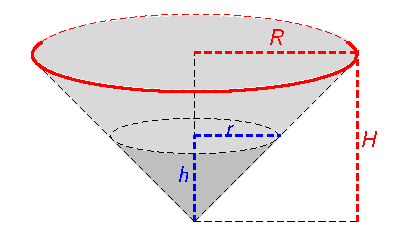
\includegraphics[scale=0.8]{22_home_antalcides_Calculo_pdf_resuelto1.pdf}
\captionsetup{,singlelinecheck=off,margin=1cm} \caption{Depósito cónico}
%
\end{minipage}%
\begin{minipage}[c]{0.55\textwidth}%
 \vspace{-4pt}
 Sabemos que $V(t)=\dfrac{1}{3}\pi\,r(t)^{2}h(t)$ donde $h(t)$ es
la altura, medida desde el vértice, alcanzada por el agua en el tiempo
$t$ y $r(t)$ es el radio de la sección transversal del cono a la
distancia $h(t)$ desde el vértice. Por semejanza de triángulos deducimos
que $\,\dfrac{r}{R}=\dfrac{h}{H}\,$, de donde, $r=r(t)=\dfrac{R}{H}h(t)=\dfrac{1}{2}h(t)$.
Luego $V(t)=\dfrac{1}{12}\pi\,h(t)^{3}$, y 
\[
V\tl(t)=\dfrac{9}{10^{3}}=\dfrac{\pi}{4}h(t)^{2}h\tl(t).
\]
%
\end{minipage}
\end{figure}
Luego, cuando $h(t_{0})=6$, deducimos que $\dfrac{9}{10^{3}}=\dfrac{\pi}{4}36h\tl(t_{0})$,
esto es, $h\tl(t_{0})=\dfrac{1}{10^{3}\pi}\ \textrm{m/sg}\ \approxeq1,146\ \textrm{m/h}$.\hecho

\resuelto El volumen de un cubo está aumentando a razón de 70\,cm$^{3}$
por minuto. ¿Con qué rapidez está aumentando el área cuando la longitud
del lado es de 12\,cm?

\sol Sea $V(t)$ el volumen del cubo, medido en centímetros cúbicos,
en el tiempo $t$, medido en minutos. Si $L(t)$ es la longitud en
centímetros del lado en el tiempo $t$, tenemos que $V(t)=L(t)^{3}$,
de donde, $L\tl(t)=\dfrac{V\tl(t)}{3L(t)^{2}}$. Como nos dicen que
$V\tl(t)=70$ cm/min, deducimos que cuando $L(t_{0})=12$, $L\tl(t_{0})=\dfrac{70}{3(12)^{2}}$.
El área del cubo viene dada por $S(t)=6L(t)^{2}$, deducimos que $\,S\tl(t_{0})=12L(t_{0})L\tl(t_{0})=\dfrac{70}{3}$
cm$^{2}$/min.\hecho

\resuelto Un barco $A$ se desplaza hacia el oeste con una velocidad
de 20 millas por hora y otro barco $B$ avanza hacia el norte a 15
millas por hora. Ambos se dirigen hacia un punto $O$ del océano en
el cual sus rutas se cruzan. Sabiendo que las distancias iniciales
de los barcos $A$ y $B$ al punto $O$ son, respectivamente, de 15
y de 60 millas, se pregunta: ¿A qué velocidad se acercan (o se alejan)
los barcos entre sí cuando ha transcurrido una hora? Y cuando han
transcurrido 2 horas? ?`En qué momento están más próximos uno de otro?

\sol Tomamos el punto $O$ como origen de coordenadas, tal como se
indica en la figura. Llamemos $x(t)$ a la distancia, medida en millas,
que separa el barco $A$ de $O$. Nos dicen que $x(0)=15$ y $x\tl(t)=-20$
millas por hora. Observa que como la función $x(t)$ es decreciente
su derivada debe ser negativa. Análogamente, sea $y(t)$ la distancia
que separa al barco $B$ de $O$.

\begin{figure}[ht]
\centering{}%
\begin{minipage}[c]{0.4\textwidth}%
\begin{center}
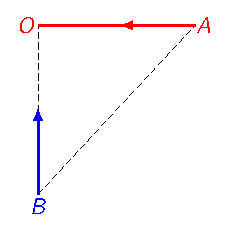
\includegraphics{23_home_antalcides_Calculo_pdf_resuelto2.pdf}
\par\end{center}
\captionsetup{,singlelinecheck=off,margin=1cm} \caption{Cruce de barcos}
%
\end{minipage}%
\begin{minipage}[c]{0.55\textwidth}%
 \vspace{-4pt}
 Nos dicen que $y(0)=60$ y $y\tl(t)=-15$ millas por hora. La distancia
entre los dos barcos viene dada por $\,f(t)=\sqrt{x(t)^{2}+y(t)^{2}}$.
Tenemos 
\[
f\tl(t)=\frac{x(t)x\tl(t)+y(t)y\tl(t)}{\sqrt{x(t)^{2}+y(t)^{2}}}
\]
Cuando ha pasado una hora $x(1)=15-20=-5$, $y(1)=60-15=45$. Deducimos
que 
\[
f\tl(1)=\frac{(-5)(-20)+45(-15)}{\sqrt{(-5)^{2}+(45)^{2}}}=-\frac{115}{\sqrt{82}}\ textrm{millas/h}
\]
Donde el sigo negativo indica que se están acercando (la distancia
entre ellos está disminuyendo). %
\end{minipage}
\end{figure}

\vspace*{10mm}

Cuando han pasado dos horas $x(2)=15-40=-25$, $y(2)=60-30=30$. Deducimos
que 
\[
f\tl(2)=\frac{(-25)(-20)+30(-15)}{\sqrt{(-25)^{2}+(30)^{2}}}=\frac{10}{\sqrt{61}}\ textrm{millas/h}
\]
Donde el sigo positivo indica que se están alejando (la distancia
entre ellos está aumentando).

La distancia entre los dos barcos es mínima cuando la derivada es
nula (fíjate que la derivada pasa de negativa a positiva). La condición
$\,f\tl(t_{0})=0$ equivale a la igualdad $-20\,x(t_{0})-15y(t_{0})=0$.
Sustituyendo en ella $x(t_{0})=15-20\,t_{0}$, $\,y(t_{0})=60-15\,t_{0}$,
obtenemos $t_{0}=\frac{48}{25}$. $x(\frac{48}{25})=-\frac{117}{5}$,
$y(\frac{48}{25})=\frac{156}{5}$. La distancia mínima a que se cruzan
los barcos es $f(\frac{48}{25})=39$ millas.\hecho

\resuelto Una bola esférica de hielo se está derritiendo de forma
uniforme en toda la superficie, a razón de 50\,cm$^{3}$ por minuto.
?`Con qué velocidad está disminuyendo el radio de la bola cuando este
mide 15\,cm?

\sol El volumen de la bola en el instante $t$ minutos viene dado
por $\,V(t)=\dfrac{4}{3}\pi\,r(t)^{3}$ centímetros cúbicos. Nos dicen
que $\,V\tl(t)=-50$. Deducimos que $-50=4\,\pi\,r(t)^{2}r\tl(t)$.
Si $r(t_{0})=15$, se sigue que 
\[
r\tl(t_{0})=\dfrac{-50}{4\,\pi(15)^{2}}=-\dfrac{1}{18\,\pi}\ \ textrm{cm/min}
\]
La derivada es negativa, como debe ser, ya que el radio está disminuyendo.\hecho

\resuelto Calcula $(f\circ g)^{\prime}(x)$ en el valor indicado
de $x$ en los siguientes casos: 

{[}a){]} 
\begin{enumerate}
\item $\dis{f(x)=\frac{2x}{x^{2}+1},\quad g(x)=10x^{2}+x+1,\quad x=0}$ 
\item $\dis{f(x)=\left(\frac{x-1}{x+1}\right)^{2},\quad g(x)=\frac{1}{x^{2}}-1,\quad x=-1}$ 
\end{enumerate}
\sol Este ejercicio lo puedes hacer de dos formas: calculando en
caso la función compuesta $(f\circ g)(x)$ y derivándola, o aplicando
la regla de la cadena sin necesidad de calcular previamente la función
compuesta. Esta segunda forma es mucho más rápida. Las derivadas que
nos piden son las siguientes.

\emph{a)}\ $f\tl(x)=\dfrac{2-x^{2}}{(x^{2}+1)^{2}},\ g\tl(x)=20x+1\;\longrightarrow\;(f\circ g)^{\prime}(0)=f\tl(g(0))g\tl(0)=f\tl(1)g\tl(0)=\dfrac{1}{4}.$
El otro apartado se hace igual.\hecho

\resuelto Calcula en cada caso el valor de $a$ y $b$ en función
de $c$, para que exista la derivada en el punto $c$ de cada una
de las siguientes funciones: 
\[
f(x)=\left\{ \begin{array}{ll}
x^{2}, & x\le c\\
ax+b, & x>c
\end{array}\right.\ \ f(x)=\left\{ \begin{array}{ll}
\dfrac{1}{\abs{x}}, & \abs{x}>c\\
a+bx^{2}, & \abs{x}\le c
\end{array}\right.\ \ f(x)=\left\{ \begin{array}{ll}
\cos x, & x\le c\\
ax+b, & x>c
\end{array}\right.
\]
\sol Consideremos la segunda de las funciones anteriores. Tenemos
que $f(x)=\frac{1}{\abs{x}}$ para $x<-c$ o $x>c$, y $f(x)=a+bx^{2}$
para $-c\le x\le c$. Imponemos primero la condición de que $f$ sea
continua en $c$. Tenemos que $f(c)=a+bc^{2}=\limlft{f(x)}{x}{c}$,
y $\limrgt{f(x)}{x}{c}=\frac{1}{\abs{c}}=\frac{1}{c}$. Debemos imponer
la condición $a+bc^{2}=\frac{1}{c}$. Impondremos también la condición
de que los límites laterales en $c$ de la derivada de $f$ coincidan.
Para $x>c$ es $f(x)=\frac{1}{x}$, por lo que 
\[
\limrgt{f\tl(x)}{x}{c}=\limrgt{-\frac{1}{x^{2}}}{x}{c}=-\frac{1}{c^{2}}.
\]
Análogamente 
\[
\limlft{f\tl(x)}{x}{c}=\limlft{2bx}{x}{c}=2bc.
\]
Debemos imponer la condición $2bc=-\frac{1}{c^{2}}$. Deducimos que
$b=-\frac{1}{2c^{3}}$ y $a=-bc^{2}+\frac{1}{c}=\frac{3}{2c}$.

Observa que las condiciones que hemos obtenido son necesarias para
que $f$ sea derivable en $c$. Pero dichas condiciones también son
suficientes como consecuencia de la proposición \ref{prop:dernodisc}.
No es necesario, por ello, que comprobemos que, con los valores de
$a$ y de $b$ obtenidos antes, efectivamente $f$ es derivable en
$c$.

Las otras dos funciones se estudian de la misma forma.\hecho

\resuelto ¿Es cierta la igualdad ${\displaystyle f\tl(a)=\lim_{t\to a}\dfrac{f(a+t)-f(a-t)}{2t}}$?
Justifica tu respuesta.

\sol Tenemos que 
\begin{align*}
\dfrac{f(a+t)-f(a-t)}{2t} & =\dfrac{f(a+t)-f(a)}{2t}+\dfrac{f(a)-f(a-t)}{2t}=\\
 & =\dfrac{1}{2}\dfrac{f(a+t)-f(a)}{t}+\dfrac{1}{2}\dfrac{f(a-t)-f(a)}{-t}
\end{align*}
Y basta tener en cuenta que: 
\[
\lim_{t\to a}\dfrac{f(a+t)-f(a)}{t}=\lim_{t\to a}\dfrac{f(a-t)-f(a)}{-t}=f\tl(a)
\]
\hecho

\resuelto Supongamos que las funciones $f$ y $g$ y sus derivadas
tienen los siguientes valores en $x=2$ y $x=3$.
\begin{center}
\begin{tabular}{|c|c|c||c|c|}
\hline 
$x$ &
$f\left(x\right)$ &
$g\left(x\right)$ &
$f\tl\left(x\right)$ &
$g\tl\left(x\right)$\tabularnewline
\hline 
\hline 
2 &
8 &
2 &
$\frac{1}{3}$ &
-3\tabularnewline
\hline 
3 &
3 &
-4 &
$2\pi$ &
5\tabularnewline
\hline 
\end{tabular}
\par\end{center}

Calcular las derivadas de las siguientes funciones en los valores
dados de $x$:

\begin{tabular}{ll}
a)\ $f(x)g(x),\quad x=3\qquad\quad$  &
b)$\ f(x)/g(x),\quad x=3$\tabularnewline
c)\ $f(g(x)),\quad x=2$  &
d)\ $\sqrt{(f(x))^{2}+(g(x))^{2}},\quad x=2$ \tabularnewline
\end{tabular}

\sol a)\ $(fg)\tl(3)=f\tl(3)g(3)+f(3)g\tl(3)=-8\pi+15$.

b)\ $\left(\dfrac{f}{g}\right)^{\!\prime}(3)=\dfrac{f\tl(3)g(3)-f(3)g\tl(3)}{g(3)^{2}}=\dfrac{-8\pi-15}{16}$.

c)\ $(f\circ g)\tl(2)=f\tl(g(2))g\tl(2)=f\tl(2)g\tl(2)=-1$.

d)\ $h(x)=\dis\sqrt{(f(x))^{2}+(g(x))^{2}}$, $h\tl(2)=\dfrac{f\tl(2)f(2)+g\tl(2)g(2)}{\sqrt{(f(x))^{2}+(g(x))^{2}}}=-\dfrac{5}{3\sqrt{17}}$.\hecho

\resuelto Supongamos que $f$ es una función que verifica una desigualdad
del tipo $\abs{f(x)}\le\abs{x}^{r}$ en algún intervalo abierto que
contiene a cero, donde $r>1$. Prueba que $f$ es derivable en $0$.

\sol La desigualdad $\abs{f(x)}\le\abs{x}^{r}$, con $r>0$, implica
que $f(0)=0$. Tenemos que 
\[
\modulo{\dfrac{f(x)-f(0)}{x-0}}=\modulo{\dfrac{f(x)}{x}}\le\abs{x}^{r-1}
\]
Como $r-1>0$, se tiene que $\Lim{\abs{x}^{r-1}}{x}{0}=0$, lo que,
por la desigualdad anterior, implica que 
\[
\lim_{x\to0}\modulo{\dfrac{f(x)-f(0)}{x-0}}=0\quad\Longleftrightarrow\quad\lim_{x\to0}\dfrac{f(x)-f(0)}{x-0}=0.
\]
Luego $f$ es derivable en $0$ y $f\tl(0)=0$.

\resuelto Calcula la derivada en todo punto de la función definida
por 
\[
f(x)=\left\{ \begin{array}{ll}
x^{2}\sen\dfrac{1}{x}, & x\neq0\\
0, & x=0
\end{array}\right.
\]

\sol Para $x\neq0$ se verifica que $\abs{f(x)}=\modulo{x^{2}\sen\dfrac{1}{x}}\le x^{2}$.
Como $f(0)=0$, resulta que $\abs{f(x)}\le x^{2}$ para todo $x\in\R$.
El ejercicio anterior implica que $f$ es derivable en $0$ con $f\tl(0)=0$.
En los intervalos $]-\infty,0[$ y $]0,+\infty[$ la función dada
es derivable por ser producto y composición de funciones derivables
en dichos intervalos, y podemos calcular su derivada con las reglas
de derivación usuales: 
\[
f\tl(x)=2x\sen\dfrac{1}{x}-\cos\dfrac{1}{x}
\]
Observa que esta derivada tiene una discontinuidad esencial en $0$.\hecho

\resuelto Calcula los puntos en que la cúbica $y=ax^{3}+bx^{2}+cx+d$,
donde $a,b,c,d$ son constantes reales, tiene tangente horizontal.
Debes estudiar los distintos casos posibles.

\sol La tangente es horizontal en los puntos donde se anula la derivada,
esto es, en las soluciones reales de la ecuación $\,3ax^{2}+2bx+c=0$,
las cuales viene dadas por 
\[
\dfrac{-2b\pm\sqrt{4b^{2}-12ac}}{6a}
\]
Si el discriminante $4b^{2}-12ac<0$ no hay ninguna solución real.
Si $4b^{2}-12ac=0$ hay una solución real doble (en la que también
se anula la derivada segunda pero no se anula la derivada tercera,
es un punto de inflexión). Si $4b^{2}-12ac>0$ hay dos puntos de tangencia
horizontal.\hecho

\resuelto Calcula un punto $c$ por la condición de que la tangente
a la parábola $f(x)=x^{2}+\alpha x+\beta$ en el punto $(c,f(c))$,
sea paralela a la cuerda que une dos puntos dados $A=(a,f(a))$ y
$B=(b,f(b))$.

\sol Dos rectas en el plano son paralelas cuando tienen igual pendiente.
Debemos calcular $c$ por la condición {\scalefont{.9}{
\[
\frac{f(b)-f(a)}{b-a}=f\tl(c)\ \Longleftrightarrow frac{b^{2}-a^{2}+\alpha(b-a)}{b-a}=2c+\alpha\ \Longleftrightarrow\ b+a+\alpha=2c+\alpha\ \Longleftrightarrow\ c=\frac{a+b}{2}
\]
}} \hecho \resuelto Calcula las ecuaciones de las rectas tangente
y normal a una hipérbola de ecuación cartesiana $y^{2}-x^{2}=1$,
en un punto genérico $(u,v)$ de la misma.

\sol Podemos expresar $y$ como función de $x$. Tenemos que $y^{2}=1+x^{2}$,
lo que da lugar a dos curvas $f(x)=\sqrt{1+x^{2}}$ (la parte de la
hipérbola en el semiplano superior $y>0$) y $g(x)=-\sqrt{1+x^{2}}$
(la parte de la hipérbola en el semiplano inferior $y<0$). La tangente
en un punto $(u,v)$ con $v=f(u)>0$ es la recta de ecuación: 
\[
y=f(u)+f\tl(u)(x-u)=v+\dfrac{u}{\sqrt{1+u^{2}}}(x-u)=v+\dfrac{ux-u^{2}}{v}\ \Longleftrightarrow\ vy-ux=1
\]
La tangente en un punto $(u,v)$ con $v=g(u)<0$ es la recta de ecuación:
\[
y=g(u)+g\tl(u)(x-u)=v-\dfrac{u}{\sqrt{1+u^{2}}}(x-u)=v+\dfrac{ux-u^{2}}{v}\ \Longleftrightarrow\ vy-ux=1
\]
En cualquier caso se obtiene la recta de ecuación $vy-ux=1$.

Podemos proceder también sin necesidad de calcular $y$ en función
de $x$. Para ello, basta observar que si expresamos $y$ en función
de $x$ y obtenemos $y=\ff(x)$ entonces se tiene que $\ff(x)^{2}-x^{2}=1$.
Podemos derivar ahora la función $x\mapsto\ff(x)^{2}-x^{2}$ con respecto
a $x$. La derivada es $2\ff(x)\ff\tl(x)-2x$ y, como dicha función
es constante igual a 1, su derivada debe ser nula. Luego 
\[
2\ff(x)\ff\tl(x)-2x=0\quad\Longleftrightarrow\quad\ff\tl(x)=\frac{x}{\ff(x)}
\]
Por tanto la derivada en un punto $u$ viene dada por $\ff\tl(u)=\frac{u}{v}$
donde $v=\ff(u)$. En consecuencia, la tangente en el punto $(u,v)$
es la recta de ecuación: 
\[
y=v+\ff\tl(u)(x-u)=v+\frac{u}{v}(x-u)=v+\frac{ux-u^{2}}{v}\ \Longleftrightarrow\ vy-ux=1
\]
Es decir, de esta forma, sin necesidad de calcular de forma explícita
$\ff(x)$ (que da lugar a las dos funciones anteriores $f(x)$ y $g(x)$),
podemos calcular la recta tangente sin necesidad de considerar cada
caso por separado.

Para que te convenzas de que esta forma de proceder es útil, considera
la hipérbola\linebreak{}
$x^{2}-y^{2}=1$. Si ahora expresas $y$ como función de $x$ obtendrás
cuatro curvas: \linebreak{}
$y_{1}=\sqrt{x^{2}-1}$ e $y_{2}=-\sqrt{x^{2}-1}$ para ($x>1$),
y $y_{3}=\sqrt{x^{2}-1}$ e %
\mbox{%
$y_{4}=-\sqrt{x^{2}-1}$%
} para ($x<-1$). Para calcular la tangente en un punto $(u,v)$ de
dicha hipérbola no merece la pena considerar cada una de ellas por
separado. Razonando como antes, se tiene que de cualquier forma que
expresemos $y=\ff(x)$ por la condición de que $x^{2}-\ff(x)^{2}=1$,
la derivada viene dada por $\ff\tl(x)=x/\ff(x)$. Por tanto la ecuación
de la recta tangente en $(u,v)$ viene dada por: 
\[
y=v+\ff\tl(u)(x-u)=v+\frac{u}{v}(x-u)=v+\frac{ux-u^{2}}{v}\ \Longleftrightarrow\ ux-vy=1
\]
\hecho \resuelto Calcula las ecuaciones de las rectas tangente y
normal a una elipse de ecuación $\dfrac{x^{2}}{a^{2}}+\dfrac{y^{2}}{b^{2}}=1$
en un punto $(u,v)$ de la misma.

\sol Procediendo como en el ejercicio anterior debes obtener la recta
de ecuación 
\[
\frac{ux}{a^{2}}+\frac{vy}{b^{2}}=1
\]
\hecho \end{ejercicios resueltos} 
